\documentclass[bachelor, och, labwork]{shiza}

\usepackage[utf8]{inputenc}
\usepackage{graphicx}

\usepackage[sort,compress]{cite}
\usepackage{amsmath}
\usepackage{amssymb}
\usepackage{amsthm}
\usepackage{fancyvrb}
\usepackage{longtable}
\usepackage{array}
\usepackage[english,russian]{babel}
\usepackage{minted}

\usepackage{tempora}


% \usepackage[colorlinks=false]{hyperref}


\newcommand{\eqdef}{\stackrel {\rm def}{=}}


\begin{document}

\title{Алгоритмы алгебры и теории чисел}

\course{4}

\group{431}

\napravlenie{10.05.01 "--- Компьютерная безопасность}


\author{Никитина Арсения Владимировича}


\satitle{доцент}
\saname{А.\,С.\,Гераськин}


\date{2022}

\maketitle

% Включение нумерации рисунков, формул и таблиц по разделам
% (по умолчанию - нумерация сквозная)
% (допускается оба вида нумерации)
%\secNumbering


\tableofcontents

\section{Задание лабораторной работы}

Осуществить проверку чисел на простоту с помощью свойств чисел Кармайкла

\section{Теоретическая часть}

\subsection{Теоремы Бигера и Дюпарка}

В 1956 году Бигер доказал, что если для простых чисел 
$p, q, r$ выполняется соотношение $p<q<r$ и $pqr$ --- число Кармайкла, то $q < 2p^2$ и $r<p^{3}$. 
Таким образом, количество чисел Кармайкла, получаемых произведением трёх простых 
множителей, один из которых известен, конечно.

Дюпарк позже обобщил этот результат, чтобы показать, что 
если $n=mqr$ --- число Кармайкла, где $q$ и $r$ --- простые, тогда 
$q<2m^{2}$ и $r<m^{3}$. Следовательно, существует не более чем конечное 
количество чисел Кармайкла со всеми, кроме двух, определёнными множителями.

Случай $m = 1$ показывает, что любое кармайклово число содержит как минимум 3 
простых множителя, к этому выводу впервые пришёл сам Кармайкл.

Итак, для того, чтобы показать, что число, проверяемое с помощью теста Ферма на
простоту было действительно простым, то требуется показать, что у данного числа
не найдется как минимум один простой делитель.


\section{Практическая часть}
\subsection{Пример работы алгоритма}
\begin{figure}[H]
    \centering
    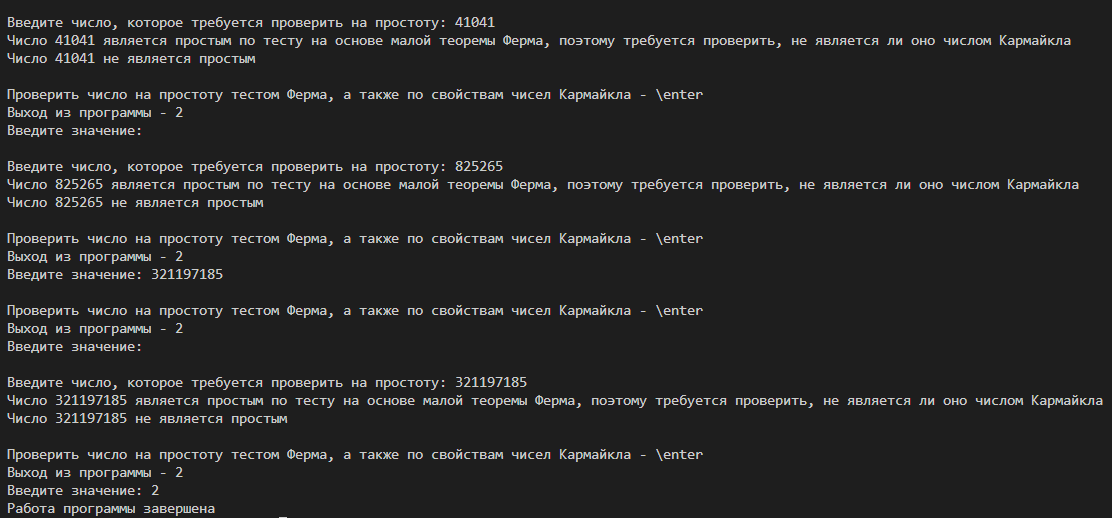
\includegraphics[width=1.0\textwidth]{pic1.png}
    \caption{}
\end{figure}

\setminted[python]{linenos,breaklines=true, fontsize=\small, style=bw}
    \subsection{Код программы, реализующей рассмотренный алгоритм}
        \inputminted{python}{lab5.py}

\end{document}